% 2961w - 30p

\documentclass[12pt,letterpaper]{article}
\usepackage{natbib}
\usepackage{pdflscape}
\usepackage{fullpage}
\usepackage{url}
\usepackage{epsfig}
\usepackage{caption}
\usepackage{hyperref}
\usepackage{enumerate}
\usepackage{dcolumn}
\usepackage{lineno}
\usepackage[T1]{fontenc}
\usepackage{textcomp}
\usepackage{float}
\restylefloat{table}
\newcolumntype{d}[1]{D{.}{.}{#1}}

\pagenumbering{arabic}


%Pagination style and stuff
\linespread{2}
\raggedright
\setlength{\parindent}{0.5in}
\setcounter{secnumdepth}{0} 
\renewcommand{\section}[1]{%
\bigskip
\begin{center}
\begin{Large}
\normalfont\scshape #1
\medskip
\end{Large}
\end{center}}
\renewcommand{\subsection}[1]{%
\bigskip
\begin{center}
\begin{large}
\normalfont\itshape #1
\end{large}
\end{center}}
\renewcommand{\subsubsection}[1]{%
\vspace{2ex}
\noindent
\textit{#1.}---}
\renewcommand{\tableofcontents}{}
%\bibpunct{(}{)}{;}{a}{}{,}

%---------------------------------------------
%
%       START
%
%---------------------------------------------

\newcommand{\disp}{\texttt{dispRity} }

\begin{document}

%Running head
\begin{flushright}
Version dated: \today
\end{flushright}
\bigskip
\noindent RH: dispRity package.

\bigskip
\medskip
\begin{center}

\noindent{\Large \bf \disp: a modular \texttt{R} package for measuring disparity.} 
\bigskip

\noindent {\normalsize \sc Thomas Guillerme$^{1,2,*}$}\\
\noindent {\small \it 
$^1$Imperial College London, Silwood Park Campus, Department of Life Sciences, Buckhurst Road, Ascot SL5 7PY, United Kingdom.\\
$^2$School of Biological Sciences, University of Queensland, St. Lucia, Australia.\\}

\end{center}
\medskip
\noindent{*\bf Corresponding author.} \textit{guillert@tcd.ie}\\  
\vspace{1in}

%Line numbering
\modulolinenumbers[1]
\linenumbers

%---------------------------------------------
%
%       ABSTRACT
%
%---------------------------------------------

\newpage
\begin{abstract} 

    \begin{enumerate}
        \item Biological data is multivariate in essence: many traits in organisms co-vary with each other in space and time.
        This causes biologists to either reduce these to a manageable number of variables or, increasingly, to use multivariate toolkits.
        One such toolkit is based on creating a multidimensional space where the variables are the axes.
        It is then possible to measure diverse aspects of the distribution of some observation (e.g. species) in this space.
        For example, if studying morphology, one can create a morphospace for two groups of species, measure the volume occupied by each of these groups and then test whether these two volumes are significantly different or not.

        \item There are as many definitions of these multidimensional spaces, metrics and tests as there are questions that can be tackled with such methods.
        Many of these methods are implemented in specific software or R packages.
        However, the definition of the space, metric and test is often dependent on the software/package authors points of view or specific questions.
        This can unfortunately hamper researchers' ability to apply different methods that best suits their specific questions.

        \item Here I present the \disp package, a flexible \texttt{R} package for performing multidimensional analysis.
        It allows users to define each step of the analysis (whether it is the space, the metric or the test) through a highly modular architecture where each definition can be passed as a function.
        It also provides a tidy interface through the \disp object, allowing users to easily run reproducible multivariate analysis.

        \item The \disp package also comes with an extend manual regularly updated following users' questions or suggestions.
        Furthermore, the package contains some simulation tools (e.g to simulate complex multidimensional space or morphological data).
        Finally, it also contains a suite of utility functions to work with \disp objects aimed at helping users to develop their own multidimensional metrics and/or tests.

    \end{enumerate}

\end{abstract}

\noindent (Keywords: disparity, ordination, multidimensionality, disparity-through-time, palaeobiology, ecology)\\

\vspace{1.5in}

\newpage 

%---------------------------------------------
%
%       INTRODUCTION
%
%---------------------------------------------

\section{Introduction}

% Multidimensionality
Biological data are complex.
To understand the ecology and evolution of species we must use multiple variables that inevitably covary with each other through time and space.
One solution to this problem is to analyse these data in a multivariate framework \citep[e.g.][]{price2015predation,diaz2016global}.
Such analyses aim to capture the complex multidimensionality of biological data, while still providing outputs that are interpretable.
These multivariate analyses can be used to investigate changes in morphological diversity through time \citep[e.g.][]{Close2015}, competitive replacement scenarios \citep[e.g.][]{Brusatte12092008}, relationships among form and function \citep[e.g.][]{diaz2016global} and even to describe the entirety of possible shapes for a group of organisms \citep[e.g.][]{raup1966geometric}.
The biological variables in such analyses are equally diverse, including morphological traits (discrete traits like the presence or absence of a character, e.g. \citealt{Close2015}; or continuous traits such as lengths, e.g. \citealt{price2015predation}), life history traits \citep[e.g.][]{diaz2016global}, or even ecosystem properties \citep[e.g.][]{DonohueDim}. 

In all these analysis, each set of multivariate traits forms a multidimensional space.
This space is represented as a matrix where rows are regarded as samples or observations (e.g. specimens, field sites, etc.) and columns are variables or some transformation thereof (e.g. embedding, scaling, ordination, etc.).
These multidimensional spaces can be defined in many ways, for example as a pairwise distance matrix (\citealt{lloyd2016estimating} and references therein; e.g. in \citealt{Close2015}), or as outputs from an ordination, whether it being a principal components analysis (PCA,
\citealt{PCA}; e.g. in \citealt{zelditch2012geometric} ), a metric scaling (PCO, PCoA, \citealt{PCO} ; e.g. in \citealt{Brusatte12092008} ) or a non-metric scaling (MDS, NMDS, \citealt{MDS}
; e.g. in \citealt{Liow2004,DonohueDim}).
The name we give to the multidimensional space tends to vary with the kinds of traits used to construct it. 
For example, when using morphological traits, the space will be a morphospace, when using ecological traits it may be referred to as an ecospace, etc.

One can then measure how the observations are distributed within this space to answer related questions (e.g. ``does group A occupy more space than group B?'').
This requires the definition of a proxy for space occupancy: the disparity metric \citep[or index;][]{Hopkins2017} which can be measured in a multitude of ways.
For example, one could use a metric based on the variance or the range of each axis of space \citep{Wills2001, Ciampaglio2001}, a distance (e.g. Euclidean) measured between observations \citep{foote1993contributions,Foote29111996}, a more direct approximation of the hyper volume \citep{cornwell2006trait,DonohueDim}, or many more \citep[e.g.][]{navarro2003MDA}.

Finally, all these different multidimensional spaces and their associated disparity metrics can be used in an equal variety of statistical tests such as non-parametric multivariate analyses of variance (NPMANOVA, \citealt{NPMANOVA}; e.g. in \citealt{Brusatte12092008}) multidimensional permutation tests (\citealt{ManlyPermutations}; e.g. in \citealt{diaz2016global}) or even, less rigorously, by looking at the confidence interval overlaps between disparity measurements.
In summary, there are many different ways to perform each step of a multidimensional analysis, making analyses of complexity ever more complex.

In theory, this multitude of ways to generate and define multidimensional spaces, measure disparity within and analyse these metrics is not an issue, in fact, it allows researchers to choose both the most appropriate method for their question or data, or even to test their question using multiple methods.
In practice, however, this is hampered by existing software implementations.
Although many software packages exist for multidimensional analysis \citep[e.g.][]{navarro2003MDA,bouxin2005ginkgo,de2007ginkgo,oksanen2007vegan,geiger2008,adams2013geomorph,Claddis,adams2017geometric},
package maintainers/software developers choose their preferred definition of multidimensional space and disparity metric to best fit their needs (i.e. data, hypothesis, etc.) making the implementations sometimes hard to adapt to different needs.
For example, in the excellent and widely used \texttt{geomorph} package, morphological disparity analysis uses the \texttt{morphol.disparity} function that defines the multidimensional space as the ordination of the Procrustes transform of the morphometric data, the disparity metric
as the relative sum of the diagonal of the covariance of the ordination scores (Procrustes variance)
, and uses permutation tests \citep{zelditch2012geometric,adams2013geomorph,adams2017geometric}.
This is ideal for testing volume based hypothesis (e.g. ``does groups A and B have the same volume?''), but in other cases may not be appropriate in non-volume based hypothesis (e.g. ``do they occupy the same location?'').
This can lead to inappropriate analyses by users confined by the existing software implementations.

The aim of the \disp package is avoid such problems by providing a flexible framework for studying multidimensional data.
This package is based on a modular architecture where each decision in multidimensional analysis (which data, metric and test) can be specified by the user.
It implements many commonly used disparity metrics, as well as providing a simple interface for users to implement their own disparity functions.
The package is described here for the use of discrete morphological data disparity analysis but can be generalised to any type of multidimensional data (see the glossary Table \ref{Tab:terms}).

\begin{table}
    \begin{tabular}{p{4cm}p{5cm}p{6cm}p{6cm}}
        \hline
        \textbf{in this manuscript} & \textbf{in} \texttt{\textbf{dispRity}} & \textbf{in palaeobiology} & \textbf{in ecology} \\ 
        \hline
        multidimensional space & matrix ($n\times k$) & morphospace, traitspace, etc. & ecospace, function-space, etc. \\
        \hline
        elements & rows ($n$) & taxa, specimen, etc. & taxa, field sites, environments, etc. \\
        \hline
        dimensions & columns ($k$) & ordination scores, distances, etc. & ordination scores, distances, etc. \\
        \hline
        subsets & matrix ($m \times k$, with $m \leq n$) & e.g. every element in a stratum or sharing the same ancestor & e.g. elements living in the same environment \\
        \hline
        disparity & a dimension-level 1 or 2 function$^1$ & disparity: e.g. the sum of variances \citep{Wills2001}, the average pairwise distances between taxa \citep{Foote01071994}, etc. & dissimilarity: e.g. ellipsoid volume \citep{DonohueDim}, convex hull volume \citep{cornwell2006trait}, etc. \\
        \hline
    \end{tabular}
    \caption{Glossary and equivalences between this manuscript, the \texttt{dispRity} package and terms commonly used in palaeobiology or ecology. $^1$See Fig. \ref{Fig:levels}.}
    \label{Tab:terms}
\end{table}


\section{Description}
In brief, the package takes a \texttt{matrix} object (the multidimensional space), calculates a disparity metric from the space and analyse the resulting \texttt{dispRity} object through hypothesis testing and visualisation.
Some additional functions modify the space, for example by dividing it by groups or through time and/or bootstrapping it (see Fig. \ref{Fig:workflow}).
Note that the input matrix is not restricted to an ordinated matrix but can be any kind of matrix as long as its rows represent elements \citep[e.g. the space can be a distance matrix][]{Close2015}.
The matrix is always considered as the final multidimensional space to analyse and no correction is applied to it (e.g. potential corrections should be applied prior to using the \texttt{dispRity} package).

\begin{figure}[!htbp]
\centering
   %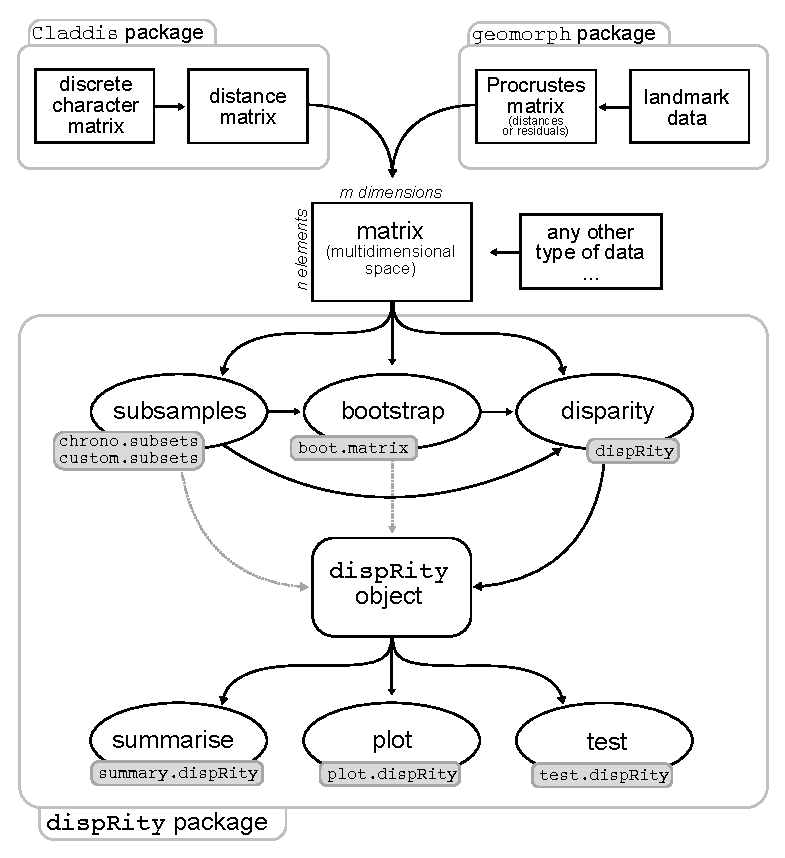
\includegraphics[width=1\textwidth]{workflowsvg.eps} 
\caption{\disp package workflow: rectangles represent matrices; ellipses represent functions; plain black arrows indicate input/output; dashed grey arrows indicate output (though the summary, plot, and test function cannot be applied if no disparity has been calculated).}
\label{Fig:workflow}
\end{figure}

\subsection{Measuring disparity}
The \disp function measures disparity from a \texttt{matrix} where the columns correspond to the dimensions and the rows correspond to the elements present in the space.
The disparity metric is passed through the \texttt{metric} argument and is defined by the user as one or more function(s) that can either transform the matrix into:

\begin{itemize}
    \item Another matrix (a dimension-level 3 function - e.g. a variance-covariance matrix; \texttt{stats::cor})
    \item A vector (a dimension-level 2 function - e.g. the variance of each dimension; \texttt{dispRity::variances} - see below)
    \item A single value (a dimension-level 1 function - e.g. the overall standard deviation; \texttt{stats::sd})
\end{itemize}

\begin{figure}[!htbp]
\centering
   %\includegraphics[width=0.8\textwidth]{dispRity_fun.eps}  %../inst/gitbook/dispRity_fun.pdf} 
\caption{Illustration of the different metric dimension-levels in the \disp package. In this example, each cell corresponds to a single value (e.g. a 8 $\times$ 7 matrix or a vector of eight elements).
A dimension-level 3 matrix would be a metric output a matrix (e.g. the function \texttt{stats::cor} to calculate the correlation between each dimension), a dimension-level 2 metric would output a vector (i.e. a distribution, e.g. \texttt{dispRity::variances} which calculates the variance within each dimension) and a dimension-level 1 metric would output a single value (e.g. \texttt{stats::sd} which calculates the standard deviation of the input matrix)}.
\label{Fig:levels}
\end{figure}

The disparity metrics can be any \texttt{R} function (see Table 2 for metrics implemented in the package).
When multiple functions are passed to the \texttt{metric} argument, they are sorted by dimension-level and applied in decreasing order to the data.
For example, if the metric is defined as \texttt{metric = c(prod, ranges)} (the hypercube volume), the \texttt{ranges} function (dimension-level 2) is first applied to data and the function \texttt{prod} is then applied to the results (\texttt{prod(ranges(data))}).
One can also directly pass a function description to the \texttt{metric} argument (e.g. \texttt{metric = function(x) mean(dist(x)$\hat{\mkern6mu}$2)} for the average squared pairwise distance).
Note that this function also allows to work on only a subset of dimensions via the \texttt{dimensions} argument (e.g. if only the $n$ first dimensions must be considered).

\begin{table}[H]
\resizebox{\textwidth}{!}
{%
    \begin{tabular}{p{2cm}|p{5cm}|p{1cm}|p{5cm}|p{5cm}}
        \textbf{name} & \textbf{description} & \textbf{dim} & \textbf{definition} & \textbf{source} \\
        \hline
        \texttt{ancestral. dist} & The distance between an element and its ancestor & 2 & $\sqrt{\sum_{i=1}^{n}{({k}_{n}-Ancestor_{n})^2}}$ & This package \\
        \hline
        \texttt{centroids} & The distance between each element and a fixed point$^1$ of the space & 2 & $\sqrt{\sum_{i=1}^{n}{({k}_{n}-Centroid_{k})^2}}$ & This package \\
        \hline
        \texttt{convhull. surface} & The surface of the convex hull & 1 & NA & \texttt{geometry::convhulln} \citep{barber1996quickhull,geometryR}\\
        \hline
        \texttt{convhull. volume} & The volume of the convex hull & 1 & NA & \texttt{geometry::convhulln} \citep{barber1996quickhull,geometryR}\\
        \hline
        \texttt{diagonal} & The greatest Euclidean distance & 1 & $\sqrt{\sum_{i=1}^{k}|max(k_i) - min(k_i)|}$ & This package \\
        \hline
        \texttt{ellipse. volume}$^2$ & The volume of the ellipsoid & 1 & $\frac{\pi^{k/2}}{\Gamma(\frac{k}{2}+1)}\displaystyle\prod_{i=1}^{k} (\lambda_{i}^{0.5})$ & This package; based on \cite{DonohueDim}\\
        \hline
        \texttt{mode.val} & The modal value & 1 & NA & This package\\
        \hline
        \texttt{n.ball. volume} & The hyper-spherical ($n$-ball) volume & 1 & $\frac{\pi^{k/2}}{\Gamma(\frac{k}{2}+1)}\displaystyle\prod_{i=1}^{k} R$ & This package\\
        \hline
        \texttt{pairwise. dist} & The pairwise distances between elements & 2 & NA & \texttt{vegan::vegdist} \citep{oksanen2007vegan}\\        
        \hline
        \texttt{radius} & The radius of each dimensions & 2 & $|\frac{\sum_{i=1}^{n}k_i}{n} - f(\mathbf{v}k)|$ & This package\\
        \hline
        \texttt{ranges} & The absolute ranges of each dimension & 2 & $|max(k_i) - min(k_i)|$ & This package \\
        \hline
        \texttt{span.tree. length} & The minimal spanning tree length & 1 & $\sum(\mathrm{branch\ length})$ & \texttt{vegan::spantree} \citep{oksanen2007vegan}\\
        \hline
        \texttt{variances} & The variance of each dimension & 2 & $\sigma^{2}{k_i}$ & This package \\
    \end{tabular}
}%
    \caption{\small{Where $k$ is the number of dimensions, $n$ the number of elements, $\Gamma$ is the Gamma distribution, $\lambda_i$ is the eigenvalue of each dimensions, $\sigma^{2}$ is their variance and $Centroid_{k}$ is their mean, $Ancestor_{n}$ is the coordinates of the ancestor of element $n$, $f(\mathbf{v}k)$ is a function to select one value from the vector $\mathbf{v}$ of the dimension $k$ (e.g. it's maximum, minimum, mean, etc.), $R$ is the radius of the sphere or the product of the radii of each dimensions ($\displaystyle\prod_{i=1}^{k}$ - for a hyper-ellipsoid). $^1$ by default that point is the centroid of the elements; $^2$ this function uses a fast estimation of the eigenvalue that only works in an ordinated space based on MDS or PCO/PCoA (\textit{not} PCA).}}
    \label{Tab:metrics}
\end{table}

\textbf{Table 2 (caption):} Where $k$ is the number of dimensions, $n$ the number of elements, $\Gamma$ is the Gamma distribution, $\lambda_i$ is the eigenvalue of each dimensions, $\sigma^{2}$ is their variance and $Centroid_{k}$ is their mean, $Ancestor_{n}$ is the coordinates of the ancestor of element $n$, $f(\mathbf{v}k)$ is function to select one value from the vector $\mathbf{v}$ of the dimension $k$ (e.g. it's maximum, minimum, mean, etc.), $R$ is the radius of the sphere or the product of the radii of each dimensions ($\displaystyle\prod_{i=1}^{k}R_{i}$ - for a hyper-ellipsoid). $^1$ by default that point is the centroid of the elements; $^2$ this function uses a fast estimation of the eigenvalue that only works in an ordinated space based on MDS or PCO (\textit{not} PCA).


\subsection{Splitting the multidimensional space into subsets}
Prior to calculating disparity, the space can be subdivided into subsets, typically to be compared to each other.
For example, one may compare the disparity of a specific subset of the space to another or, how different subsets change sequentially (e.g. through time).
The original space corresponds to the overall space (e.g. a morphospace contains all the observed morphologies).
Subsets correspond to parts of the space with pooled characteristics.

This splitting can be done using the \texttt{custom.subsets} or \texttt{chrono.subsets} functions.
The first function takes a matrix defining the space and a list of elements defining the subsets.
The second also takes a matrix and arguments giving the age of the taxa (a dated phylogeny of the elements present in the morphospace - see below) and which subsets to create: (1) discrete time subsets (or time-binning) or (2) continuous time subsets (or time-slicing).

The time-binning method groups elements by specific age range.
The time-slicing method works by using a phylogeny and looking at which taxa are present at any specific point in time.
This method thus requires the nodes to be part of the space, a dated phylogeny (chronogram) and which model to use when slicing through branches rather than tips and nodes.
When a slice occurs not on a tip or a node, six methods are available to select either the descendent or the ancestor's node/tip as an element for this time slice:
``acctran'', ``deltran'', ``random'' and ``proximity'' as proxy for punctuated evolution models; and ``equal.split'', ``gradual.split'' as a proxy for gradual evolution.
See \cite{time-slice} for full description of the method.
Note that there is a trade-off between precision and accuracy when using the time-slicing method: a higher number of slices increases the precision of the disparity analysis but also decreases accuracy.

\subsection{Bootstrapping and rarefying}
Disparity measurement can be influenced by sampling \citep{Butler2012}.
To take this source of bias into account, one can bootstrap the multidimensional space or/and to rarefy the data.
Additionally, if disparity is defined as a dimension-level 1 metric, it can be useful to measure it on bootstrapped data to obtain a distribution on which to perform statistical analyses.

Bootstrapping can be achieved by using the \texttt{boot.matrix} function which pseudo-replicates the space following two algorithms: (1) the ``full'' algorithm where the bootstrapping is entirely stochastic ($n$ elements are replaced by any $m$ elements drawn from the data); and (2) the ``single'' algorithm where $n = 1$ (similar to jackknife).

Similarly, rarefaction can be achieved through the same \texttt{boot.matrix} function.
In practice, rarefaction limits the number of elements to be drawn for each bootstrap replication: only $n-x$ elements are selected at each bootstrap replicate (where $x$ is the number of non-sampled elements).

\subsection{Interpreting results}
The functions above all generate a \disp object that can be summarised or plotted using the \texttt{S3} method functions \texttt{summary.dispRity} and \texttt{plot.dispRity}.
These results can also be analysed using the \texttt{test.dispRity} function for comparing subsets or testing hypotheses.

\subsubsection{Summarising and plotting}
The \texttt{summary.dispRity} and \texttt{plot.dispRity} functions allow users to set which central tendency and which quantiles should be represented.
The \texttt{plot.dispRity} function graphically represents the summarised results using different representations: (1) ``continuous'' for displaying continuous disparity curves and (2) ``box'', ``lines'', or ``polygons'' to display them using boxplots, confidence interval lines or polygons respectively.
Additional arguments specific to \disp objects can also be used such as \texttt{observed} to display the observed disparity (i.e. non-bootstrapped) or \texttt{rarefaction} to only plot the disparity for a certain number of elements (i.e. the rarefaction level).
The function can also take any additional graphic arguments (\texttt{main}, \texttt{xlab}, \texttt{col}, etc...) from base \texttt{R}.

\subsubsection{Testing hypotheses}
The \texttt{test.dispRity} function allows users to test hypotheses on the disparity data.
Similarly to the \disp function described above, this function can take any test defined by the user or from other R packages.
The \texttt{comparison} arguments indicates in which order (if any) the tests should be applied to the subsets: (1) ``pairwise'' for pairwise comparisons; (2)``referential'' for comparing the first subset to all the others; (3) ``sequential'' for comparing subsets sequentially (e.g. first against second, second against third, etc.); (4) ``all'' for comparing all the subsets simultaneously (i.e. \texttt{disparity $\mathtt{\sim}$ subsets}) or (5) any list of pairs of subsets to compare.

Some tests are implemented within the package such as the Bhattacharrya Coefficient \citep[\texttt{bhatt.coeff};][]{Bhattacharyya,GuillermeCooper}, a permutation test based on null hypothesised multidimensional space following \cite{ManlyPermutations,diaz2016global} (\texttt{null.test}) 
as well as a wrapper for the \texttt{vegan::adonis} \citep{oksanen2007vegan} and \texttt{geiger::dtt} \citep{geiger2008} functions (respectively \texttt{adonis.dispRity} and \texttt{dtt.dispRity}).
This function also allows additional arguments such as \texttt{rarefaction} (as described above) or \texttt{correction} to adjust p-values when using multiple parametric tests.

\section{Examples}
Multivariate analysis can be really useful for looking at multiple aspects of organisms' diversity together.
For example, one can also look the diversity of morphologies \citep[or disparity;][]{foote1991morphological}.
Using disparity, it is then also possible to assess whether one ecosystem or/and time period display more morphological variation.
The following example is based on a classical morphological disparity analysis.
Note that more examples are available in the package manual (\url{https://rawgit.com/TGuillerme/dispRity/master/inst/gitbook/_book/index.html}).

\subsubsection{\disp data}
The package contains a dataset that is a subset from \cite{beckancient2014} and includes:

\begin{itemize}
    \item \texttt{BeckLee\_mat50}: an ordinated matrix for 50 mammals based on the distance between discrete morphological characters.
    \item \texttt{BeckLee\_mat99}: the same matrix \texttt{BeckLee\_mat50} with the reconstruction of their 49 ancestors.
    \item \texttt{BeckLee\_tree}: a chronogram with the 50 mammal species present in \texttt{BeckLee\_mat50} and \texttt{BeckLee\_mat99}.
    \item \texttt{BeckLee\_ages}: the first and last occurrence data for 14 of the mammal species present in \texttt{BeckLee\_mat50} and \texttt{BeckLee\_mat99}.
    \item \texttt{disparity}: a pre-analysed \disp object based on the data above.
\end{itemize}

In this example, the space is defined as a morphospace: the ordination of the distances among discrete morphological characters for 50 mammal species \citep[from][]{beckancient2014}.
Additionally, we can define disparity as the sum of the variances on each dimension \citep{foote1991morphological,Wills1994} that will represent an aspect of the the volume of the morphospace.

\subsubsection{Typical disparity among groups analysis}
One typical question with such analysis would be to test whether two groups of species have a different disparity.
For example, using the data described above, we can test whether the crown mammals are more diverse in term of morphology than the stem ones.
In other words, whether the approximation of the volume within the morphospace is different in crown or stem mammals.
These two groups can be defined using one the package's utility functions, \texttt{crown.stem} that separate the crown and stem species given a phylogeny (allowing to ignore the nodes or not):

\noindent
\texttt{> mammal\_groups <- crown.stem(BeckLee\_tree, inc.nodes = FALSE)}

\noindent It is then possible to measure the disparity between the two groups as follows:

\noindent
\texttt{> disparity <- dispRity.per.group(data = BeckLee\_mat50,}\\
\texttt{group = mammal\_groups, metric = c(sum, variances))}

\noindent Note that this function is a wrapper function that is the equivalent to:

\noindent
\texttt{> subsets <- custom.subsets(data = BeckLee\_mat50, group = mammal\_groups)}\\
\noindent
\texttt{> bootstraps <- boot.matrix(subsets)}\\
\noindent
\texttt{> disparity2 <- dispRity(bootstraps, metric = c(sum, variances))}\\

\noindent Which allows a finer tuning of the optional arguments in each function.
The three arguments here are defined as follows: \texttt{data = BeckLee\_mat50} is our space, \texttt{group = mammal\_groups} indicates which mammals belong to which group and \texttt{metric = c(sum, variances)} is our definition of disparity \citep{foote1991morphological,Wills1994,Ciampaglio2001}. 

This function returns a \disp object that summarises the disparity analysis:

\noindent \texttt{> disparity2}\\
\noindent \texttt{ ---- dispRity object ---- }\\
\noindent \texttt{2 customised subsets for 50 elements with 48 dimensions:}\\
          \texttt{crown, stem.}\\
\noindent \texttt{Data was bootstrapped 100 times (method:"full").}\\
\noindent \texttt{Disparity was calculated as: c(sum, variances).}\\

\bigskip
As indicated, the \disp object contains two customised subsets from a morphospace made of 50 elements for 48 dimensions.
The \disp object also displays information on the number and method of the bootstrap replicates as well as the definition of disparity.
To visualise the actual disparity values, one can use the \texttt{summary} or/and \texttt{plot} options (Table \ref{Tab:summary_group} and Fig. \ref{Fig:plot_group}):


\noindent \texttt{> summary(disparity2)}

\begin{table}[ht]
\centering
\begin{tabular}{rlrrrrrrr}
  \hline
 & subsets & n & obs & bs.median & 2.5\% & 25\% & 75\% & 97.5\% \\ 
  \hline
1 & crown &  30 & 2.00 & 1.93 & 1.87 & 1.92 & 1.95 & 1.98 \\ 
  2 & stem &  20 & 1.72 & 1.63 & 1.53 & 1.60 & 1.66 & 1.69 \\ 
   \hline
\end{tabular}
\caption{Summarising a \disp object (disparity per groups). $n$ is the number of elements per subsets, $obs$ the observed disparity (not bootstrapped), $bs.median$ is the median bootstrapped disparity (here the median of the sum of variances) and the 2.5, 25, 75 and 97.5\% are the confidence intervals.}
\label{Tab:summary_group}
\end{table}

\noindent \texttt{> plot(disparity2)}

\begin{figure}[!htbp]
\centering
   %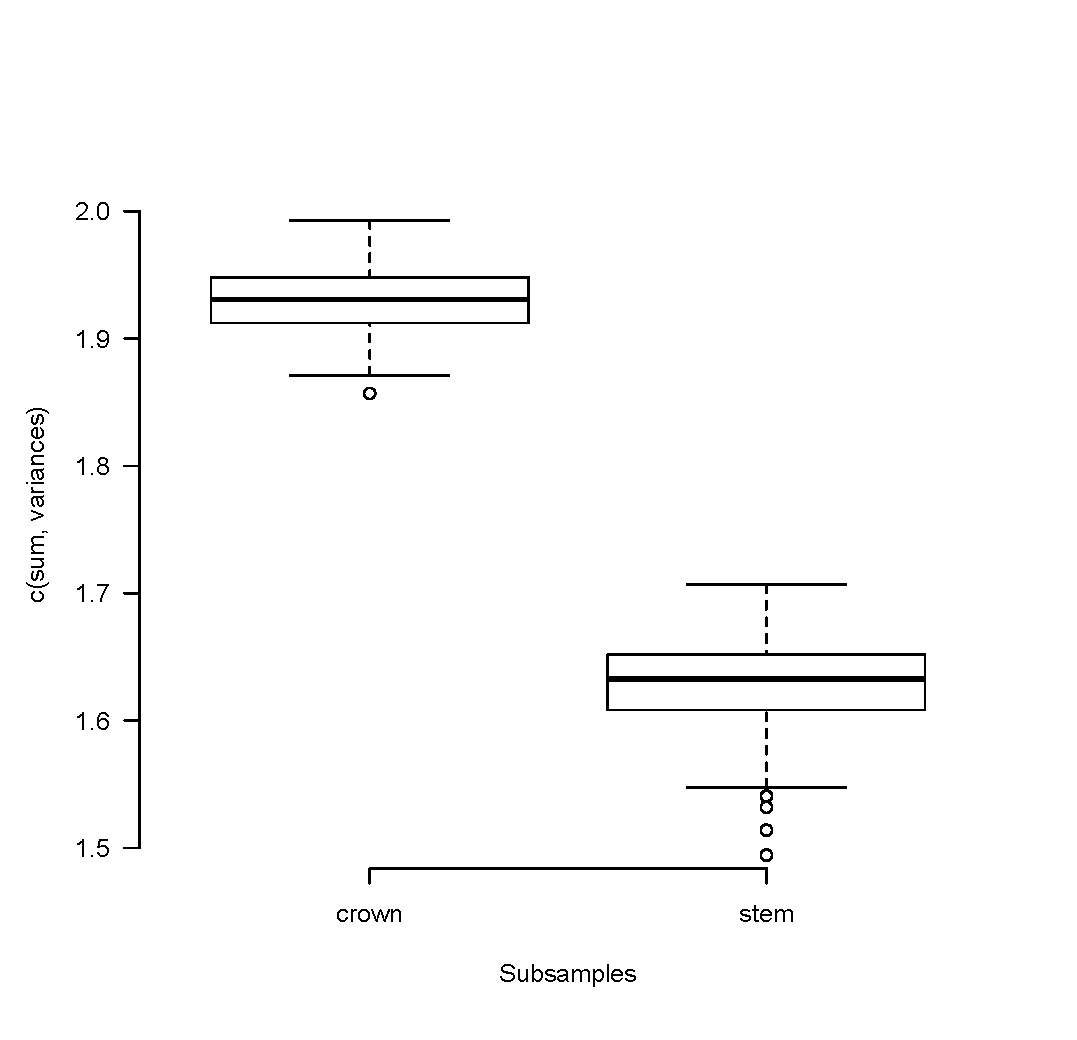
\includegraphics[width=1\textwidth]{plot_example_group.eps} 
\caption{\disp plot of disparity differences between groups.}
\label{Fig:plot_group}
\end{figure}

As we can see from the summary table (Table \ref{Tab:summary_group}) and the plot (Fig. \ref{Fig:plot_group}), there seems to be a significant difference in morphospace volume occupied between the two groups.
It is possible to test this hypothesis by using, for example, a non-parametric Wilcoxon test (\texttt{stats::wilcox.test}):

\noindent \texttt{> test.dispRity(disparity2, test = wilcox.test)}\\

\noindent \texttt{[[1]]}\\
\noindent \texttt{          statistic: W}\\
\noindent \texttt{crown : stem     10000}\\
\noindent \texttt{ }\\
\noindent \texttt{[[2]]}\\
\noindent \texttt{                  p.value}\\
\noindent \texttt{crown : stem 2.562144e-34}\\

\bigskip
As indicated by the \textit{p} value, there is a significant difference in disparity between the groups.
Note that by default the function only outputs the test's statistic, parameter (if parametric) and the \textit{p} value.
However, the raw test results can also be output using the option \texttt{details = TRUE} in the function above.
Additionally, the test is here performed on the pooled bootstrapped pseudo-replications which can increase the type I error.
It is possible to compare each bootstrap in a pairwise way without pooling the data by using the \texttt{concatenate = FALSE} argument.
The results will then be a distribution of statistics and \textit{p} values.
Relating back to our question: yes, crown mammals display a higher diversity in morphologies than their stem counterparts (in this example and dataset).

\subsubsection{Typical disparity-through-time analysis}
A subsequent question to this observation could be to test whether this difference is due to an overall change in disparity through time or not.
Using the same definition of the multidimensional space and disparity as in the previous example, we can measure, for example, changes in disparity through time between the Late Cretaceous (100.5 to 66.0 million years ago - Mya), the Paleocene (66.0 to 56.0 Mya) and the Eocene (56.0 to 33.9 Mya).
Note that stratigraphic times can be generated automatically using the \texttt{get.bin.ages} utility function.

\noindent
\texttt{> time\_bins <- c(100.5, 66, 56, 33.9)}

It is then possible to measure disparity-through-time using the following function:

\noindent
\texttt{> disparity3 <- dispRity.through.time(data = BeckLee\_mat50,}\\
\texttt{tree = BeckLee\_tree, time = time\_bins, metric = c(sum, variances))}

\noindent Note that this function is a wrapper function that is the equivalent to:

\noindent \texttt{> time\_subsets <- chrono.subsets(data = BeckLee\_mat50, tree = BeckLee\_tree,}\\ \texttt{time = time\_bins, method = \textquotedbl discrete\textquotedbl)}\\
\noindent \texttt{> bootstraps2 <- boot.matrix(time\_subsets)}\\
\noindent \texttt{> disparity4 <- dispRity(bootstraps2, metric = c(sum, variances))}\\

\noindent The arguments \texttt{data = BeckLee\_mat50} and \texttt{metric = c(sum, variances)} are the same as in the example above.
However, in this type of analysis, we also need to have additional arguments: the \texttt{time = time\_bins} indicates the boundaries of the different time bins, the \texttt{tree = BeckLee\_tree} argument provides information on the age of each element and \texttt{method = "discrete"} indicates that the data is time-binned.
The resulting \disp object can be summarised and plotted (Table \ref{Tab:summary_time} and Fig. \ref{Fig:plot_time}):

\noindent \texttt{> summary(disparity4)}

\begin{table}[ht]
\centering
\begin{tabular}{rlrrrrrrr}
  \hline
 & subsets & n & obs & bs.median & 2.5\% & 25\% & 75\% & 97.5\% \\ 
  \hline
1 & 100.5 - 66 &  15 & 1.67 & 1.55 & 1.40 & 1.51 & 1.58 & 1.65 \\ 
  2 & 66 - 56 &   9 & 1.88 & 1.69 & 1.43 & 1.63 & 1.77 & 1.83 \\ 
  3 & 56 - 33.9 &  13 & 1.96 & 1.83 & 1.62 & 1.77 & 1.86 & 1.90 \\ 
   \hline
\end{tabular}
\caption{Summarising a \disp object (disparity through time). $n$ is the number of elements per subsets, $obs$ the observed disparity (not bootstrapped), $bs.median$ is the median bootstrapped disparity (here the median of the sum of variances) and the 2.5, 25, 75 and 97.5\% are the confidence intervals.}
\label{Tab:summary_time}
\end{table}

\noindent \texttt{> plot(disparity4, type = \textquotedbl continuous\textquotedbl)}

\noindent Note that many plot options specific to \disp objects are available such as plotting disparity in a ``continuous'' fashion (inferring disparity between the time bins).

\begin{figure}[!htbp]
\centering
   %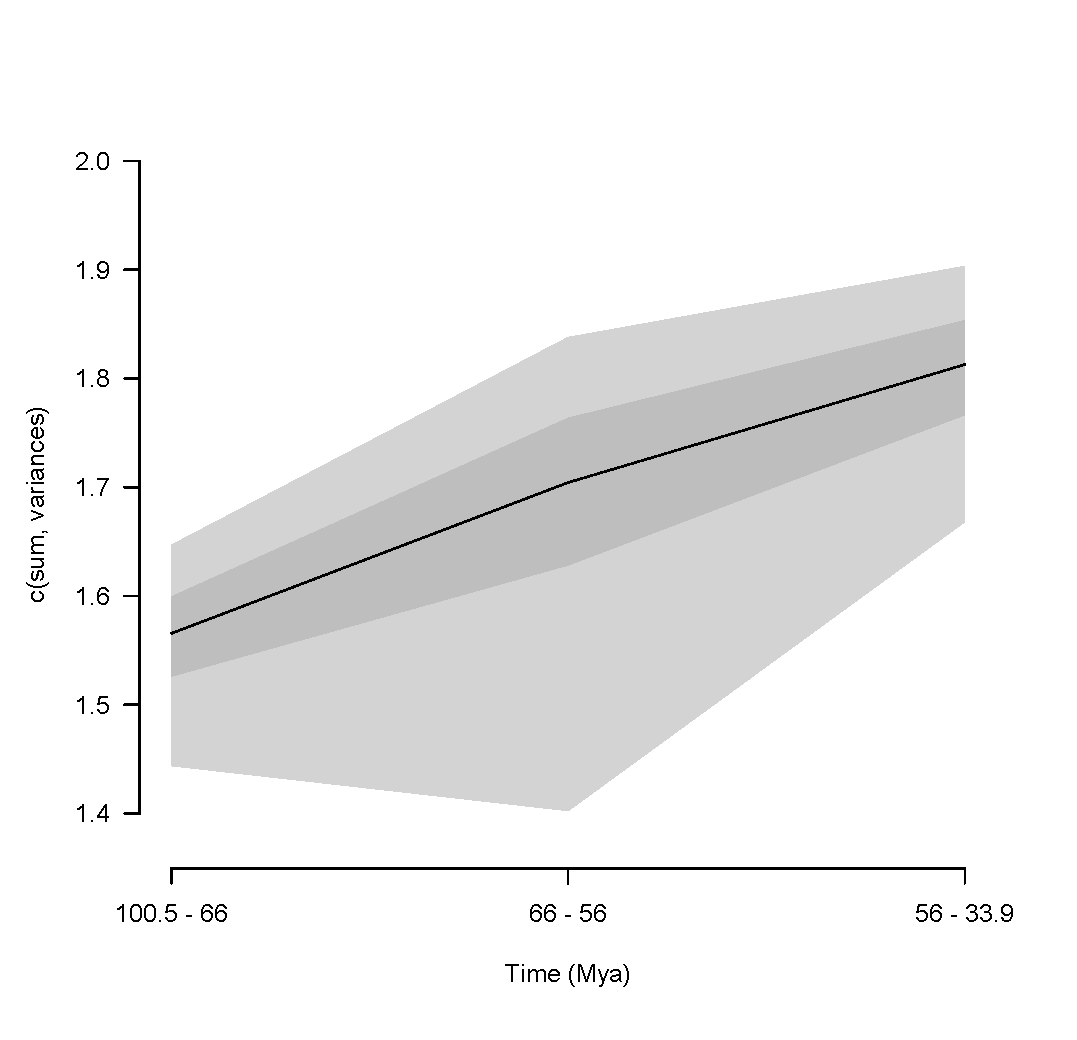
\includegraphics[width=1\textwidth]{plot_example_time.eps} 
\caption{\disp plot of disparity-through-time. The black line represents the median disparity (median sum of variances), the dark grey and light surfaces represent respectively the 50\% and 95\% confidence intervals.}
\label{Fig:plot_time}
\end{figure}

Similarly to the example above, it is also possible to statistically test this hypothesis using, for example, multivariate permutation ANOVA  \citep[PERMANOVA; ][]{NPMANOVA} through the \texttt{adonis.dispRity} function that is a wrapper of the \texttt{vegan::adonis} function  \citep{oksanen2007vegan} for \texttt{dispRity} objects:

\noindent \texttt{> test.dispRity(disparity4, test = adonis.dispRity)}

\begin{table}[ht]
\centering
\begin{tabular}{lrrrrrr}
  \hline
              & Df & Sum Sq & Mean Sq & F Model & R2   & Pr($>$F) \\ 
  \hline
    time      & 2  &  7.50 & 3.75     & 2.06    & 0.11 & <0.01 *** \\ 
    Residuals & 34 & 61.82 & 1.81     &         & 0.89 & \\
    Total     & 36 & 69.32 &          &         & 1.00 & \\ 
   \hline
\end{tabular}
\caption{
Permanova output from \texttt{adonis.dispRity}:\\
Call: vegan::adonis(formula = dist(matrix) \texttildelow time, data = disparity2, method = "euclidean"); Permutation: free; Number of permutations: 999; Terms added sequentially (first to last). Signif. codes:  0 `***' 0.001 `**' 0.01 `*' 0.05 `.' 0.1 ` ' 1.
}
\label{Tab:anova}
\end{table}

To answer our specific question above: yes, there is an effect of time on morphological disparity (an increase) in this dataset (Table \ref{Tab:anova}).
Note that in this case, the function outputs different warnings on the usage of such test and the eventual data not used in the test.
Additionally, the test is not applied to the bootstrapped data and thus might be sensitive to outliers and sampling size.

\section{Additional information}
\subsection{Manuals and vignette}
Supplementary information concerning the package and each function can be found in \texttt{R}, on the project page (
\url{https://TGuillerme/dispRity}) or in the online manual (\url{https://rawgit.com/TGuillerme/dispRity/master/inst/gitbook/_book/index.html}).
This manual contains substantially more information and detailed examples including a tutorial for a ``classic'' disparity analysis in palaeobiology as well as an introduction to the use of this package in ecology or other disciplines. 

\subsection{Data simulations}
This package also contains functions for simulating random discrete morphological matrices (\texttt{sim.morpho}) or random multidimensional spaces (\texttt{space.maker}).
These functions are based on a similar modular architecture as that used by the \texttt{dispRity} functions, allowing users to provide their own distribution parameters for the simulations.
For example, \texttt{stats::rnorm} can be provided as an argument for drawing normal characters rates with \texttt{sim.morpho} or normally distributed spaces with \texttt{space.maker}.
The discrete morphological data simulations are based on protocols from \cite{GuillermeCooper}, \cite{OReilly20160081} and \cite{puttick2017uncertain}.
The space simulations are based on the methods from \cite{diaz2016global}.
Both functionalities are described in more details in the package manual.

\section{Conclusion}
The \disp package is based on a modular architecture allowing researchers to simply define both their multidimensional space and their disparity metric to efficiently analyse multivariate data.
The \disp object allows users to pipeline disparity analysis from the data input (the matrix) to publication standard results (tables, plots, hypothesis testing).

\section{Package location}
The \disp package is available on the CRAN at \url{https://cran.r-project.org/web/packages/dispRity/index.html} or on GitHub at \url{https://github.com/TGuillerme/dispRity} with more associated information.
All the versions of the package are archived on ZENODO with associated DOI \url{https://zenodo.org/record/1186467#.WtfbGsi-kW8}.

\section{Acknowledgments}
Many thanks to Natalie Cooper for encouraging and helping with the writing of this paper and the package manuals.
Thanks to David Bapst, Martin Brazeau, Rompy Chompee, Andrew Jackson, Graeme Lloyd and Emma Sherratt and to Michael Collyer, Gavin Simpson and two other anonymous reviewers for comments on the package and manuscript.
I acknowledge support from European Research Council under the European Union's Seventh Framework Programme (FP/2007 - 2013)/ERC Grant Agreement number 311092 awarded to Martin Brazeau and from the Discovery Project Grant DP170103227 awarded to Vera Weisbecker.

\bibliographystyle{sysbio}
\bibliography{References}

\end{document}
